%----------------------------------------------------------------------------
\chapter{Rendszer felépítése}
\label{sec:system}
%----------------------------------------------------------------------------
Ebben a fejezetben szeretném bemutatni az általam elkészített rendszert és az azt alkotó egyes részeket.


%----------------------------------------------------------------------------
\section{Rendszer részei}
%----------------------------------------------------------------------------
Az elkészült rendszer három fő komponensből áll. Ezek együttesen képesek tetszőleges tulajdonsággal rendelkező szolgáltatás hálózatokat megvalósítani, azt Kubernetes alatt elindítani, forgalmat generálni és mérés során adatokat gyűjteni. 

Az egyes részekről bővebben is lesz szó, azonban most átfogóan ismertetem a rendszert, ami a \ref{fig:system_overview} ábrán látható. Minden elem megalkotásánál egy lényeges szempont volt, hogy az elkészült rendszerrel könnyen lehessen méréseket indítani és a lehető legtöbb paraméter konfigurálható legyen.

A mérések paramétereit egy konfigurációs fájlban tudjuk megadni, ahonnan egy Python program olvassa be és vezényli le a mérések elvégzését. Először a Kubernetes API-n keresztül létrehoz egy \textit{ServiceGraph} objektumot. Ez nem egy beépített típus, úgyhogy a Kubernetes nem tud vele mit kezdeni ezért írni kellett egy operátort, ami képes egy ilyen definíció szerint létrehozni a szükséges erőforrásokat (\textit{deployment, pod, service, HPA}). Ahhoz, hogy az egyes kiszolgáló egységeket is tudjuk tetszés szerint konfigurálni kell egy olyan képfájl, ami a megadott paraméterek alapján tud működni. Ezért írni kellett egy külön alkalmazást hozzá.

Miután elkészültek a kért objektumok és képesek már kiszolgálni a klaszteren kívülről érkező igényeket a Python szkript elkezd forgalmat generálni. A terhelés lejárta után ki kell nyerni a mérés során keletkezett adatokat. Ebben egy külön szoftver segít a Prometheus\citep{Prometheus}. 

Az elkészült rendszerhez szükséges részek forráskódjai megtalálhatóak a GitHub felületén\citep{gitRepo}. 

% Rendszer áttekintése -------------------------------------------------------
\begin{figure}[!ht]
\centering
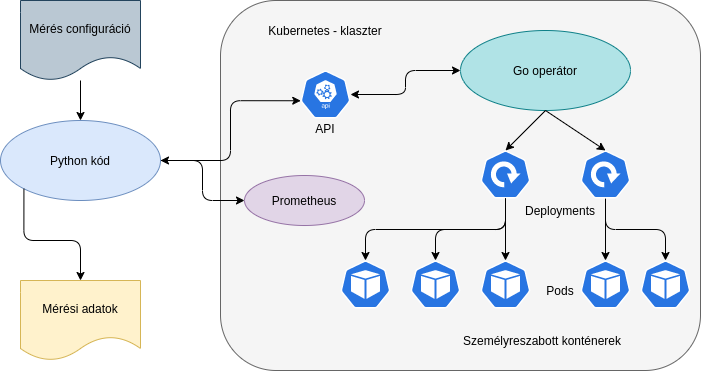
\includegraphics[width=150mm, keepaspectratio]{figures/system_overview.png}
\caption{Rendszer áttekintése}
\label{fig:system_overview}
\end{figure}

%----------------------------------------------------------------------------
\section{Korábbi munkák}
%----------------------------------------------------------------------------
A korábbi projekttárgyak keretén belül már foglalkoztam hasonló kérdéskörrel, így már volt az egyes eszközök használatához tapasztalat és implementáció is, amiből ki lehetett indulni. 
Önálló labor tárgyban megismerkedtem a Go programozási nyelvvel, és elkészítettem egy Kubernetes operátort, ami képes egyedi erőforrás definíciók feldolgozására és ez alapján képes beépített objektumokat létrehozni. A félév elején elején ezt tovább kellett bővíteni, hogy képes legyen skálázót is létrehozni valamint javítani kellett a megbízhatóságán is.

Korábban készítettem már egy Docker képfájl is, ami a jelenlegi rendszerben felhasználttal azonos céllal született, hogy szabadon konfigurálható paraméterezés alapján szolgálja ki a beérkező kéréseket. Az így megírt Go alapú webszervert is a félév során tovább kellett bővíteni, személyre szabni, hogy a valósághűbb eredményeket szolgáltasson.

%----------------------------------------------------------------------------
\section{Operátor}
%----------------------------------------------------------------------------
Fontos szempontnak tekintettük, hogy egyszerű konfigurációs fájl alapján létre lehessen hozni a szolgáltatáshálót, amit szeretnénk tesztelni.
A Kubernetes rendszer nem tartalmaz olyan erőforrást, ami számunkra ezt a funkcionalitást alapvetően támogatná.
A feladat számunkra az lesz, hogy egy közös konfiguráció alapján több különfajta, már beépített erőforrást hozzunk létre.
Már az orkesztrációs platform fejlesztésénél felkészültek arra az esetre, hogy sok egyedi igény fog megjelenni a különböző használatból fakadóan, ezért már fejlesztés közben fontos szempont volt a Kubernetes könnyű kibővítése.
A mögöttes gondolat az, hogy nagyon változó igények és funkcionalitások jelenhetnek meg a felhasználási körülményektől függően, amiket nem célszerű a központi egységbe implementálni, hiszen akkor a rendszer könnyen átláthatalanná és inkonzisztensé válna.
Helyette egyedi erőforrásokat (CustomResource) hozhatunk létre és ezen erőforrások mellé megadhatunk különöző vezérlőket. Ezt csinálják az operátorok, amivel a fentebb vázolt feladat a diplomamunkában is megoldhatóvá vált.

\subsection{Megírása}
%----------------------------------------------------------------------------
A klaszter operátorral való kibővítése egy gyakran alkalmazott megoldás, amikor összetettebb alkalmazást vagy logikát kell implementálni. Olyan szinten elterjedt megoldásról van szó, hogy több nyelv és keretrendszer közül lehet választani\citep{availableOperatorFrameworks}. Valamint külön weboldal is létezik, ahol össze vannak gyűjtve az egyes alkalmazásokhoz elérhető, korábban megírt operátorok.\citep{operatorhub} A Kubernetes alkalmazási lehetőségei között ezt a megoldást külön mintaként említik.\citep{KubernetesPatterns} 

Én a feladat megoldásához az Operator-SDK\citep{operatorSDK} keretrendszerét használtam fel. A keretrendszerrel könnyen írhatunk Kubernetes operátorokat. Ezt megtehetjük Helm, Ansible vagy Go segítségével is. Értelemszerűen a legnagyobb rugalmasságot a Go programozási nyelvvel érhetjük el, itt van lehetőségünk nagyon mély szinten belenyúlni a klaszter működébe. Én is ezt a megoldást választottam a korábbi projekttárgy keretén belül és sikerült megszerezni az alapvető ismerteket. A korábban megírt alkalmazás több hibát is tartalmazott, így a diplomamunka keretén belül ezeket ki kellett javítani és új funkciókkal bővítettem ki.

Sajnos limitált számú segédanyag érhető el és azokis többnyire ugyanazt a példaalkalmazást mutatják be, ezért az elején nehéz belekezdeni. Egyedül a korábban mások által megírt operátorok forráskódja tudott jó kiindulásként szolgálni.

Több megoldás is létezik az elkészült operátorunk futtatására. Futtathatjuk a klaszteren kívülről, mint alkalmazást, illetve a klaszteren belülről is. Utóbbi esetben készíteni kell az alkalmazásunkból egy Docker képfájlt, ami aztán külön kapszulában fog futni. Illetve klaszteren belül lehetőségünk van egy úgynevezett operátor életciklus kezelővel (Operator Lifecycle Manager - OLM) is megtenni ezt. Az utóbbi megoldás a legfejlettebb úgy kell elképzelni mint egy külön csomagkezelő csak a klaszteren belül, az operátoroknak. A félévben én a klaszteren kívüli megoldást használtam, mivel az operátort is folyamatosan fejleszteni kellett a különböző igények szerint, illetve a projekt kapcsán nem releváns az operátor futási környezete, cserébe több idő marad a mérésekre koncentrálni.

\subsection{Használata}
%----------------------------------------------------------------------------
A \ref{servicegraph_example} kódrészlet mutat egy példát a szolgáltatásháló definíciójára. Számunkra elég végiggondolni, hogy milyen szolgáltatásokat szeretnénk, hogyan kövessék egymást, milyen erőforrást biztosítsunk számukra. Miután ezek megvannak készítünk belőle egy \textit{yaml} dokumentumot.

Látható, hogy a \verb+apiVersion+ és \verb+kind+ érték egyedi, így tudunk hivatkozni a saját erőforrásunkra. Szintén meg kell adni pár meta információt, mint például az objektum neve és névtere. A \verb+spec+ szekció az érdekes számunkra. Itt tudjuk felsorolni, hogy milyen szolgáltatásokat szeretnénk majd a hálózatba. Be tudjuk állítani, hogy hány replikával fusson egy-egy szolgáltatás, illetve hogy milyen portokon tudjuk majd őket elérni. Ezek az információk azért lesznek fontosak, mert ez alapján fog az operátor létrehozni Kubernetes Deploymenteket és Serviceket. Ha szeretnénk skálázást is beállítani az adott szolgáltatásra akkor azt is megtehetjük, ha megadjuk a \verb+hpa+ konfigurációs paramétereket. Ezek hiányában nem kerül létrehozásra, és fix replikaszámmal fog üzemelni.

Továbbá definiálni kell, hogy az adott szolgáltatás milyen végpontok hívására figyeljen. Például a \textit{front-end} szolgáltatás a \verb+/instant+ és \verb+/chain+ lekérdezésekre fog válaszolni. A válasz gyorsasága és a közben felhasznált erőforrás mennyiséget is lehetőségünk van befolyásolni. Az itt megadott paraméterek továbbításra kerülnek majd a futtatott konténerekhez így ők fogják helyileg érvényre juttatni a szabályokat. 

A bemutatott kód csak részlete a teljes forrásállománynak, mert elég repetitív ezért nem szerettem volna a helyet foglalni, de a GitHub oldalán megtalálható a teljes kód. \\

\lstset{caption=Saját szolgáltatásháló definiálása, label=servicegraph_example}
\lstinputlisting{figures/servicegraph.yaml}

Miután megtörtént a szolgáltatásháló leírása és fut a korábban elkészített operátor könnyű dolgunk van. Mintha csak egy beépített erőforrást hoznánk létre a \ref{servicegraph_apply} kódrészletben mutatott módon telepíthető is. 
Ilyenkor az történik, hogy a \verb+kubectl+ parancs a Kubernetes API-t meghívja, és továbbítódik az operátor felé. Az operátor kiolvassa a kapott objektum értékeit és ez alapján létrehozza a kívánt erőforrásokat. 

\lstset{caption=Szolgáltatásháló indítása, label=servicegraph_apply}
\begin{lstlisting}[language=bash,morekeywords={kubectl, apply},alsoletter={-},breaklines=true]
$ kubectl apply -f path/to/servicegraph.yaml                          
servicegraph.dipterv.my.domain/servicegraph created 
\end{lstlisting}


%----------------------------------------------------------------------------
\section{Go konténer}
%----------------------------------------------------------------------------
A korábban látott módon lehetőségünk van tetszőleges szolgáltatásokat elindítani, azonban hogy az adott szolgáltatásoknak további paraméterek tudjunk átadni, olyan alkalmazás kell ami tudja kezelni őket. Például: milyen végpontokra figyeljenek, milyen kiszolgálási idővel dolgozzanak, mennyi erőforrást használjanak fel.
A feladat megoldására létrehoztam egy Go alapú webalkalmazást, mely induláskor átveszi a szükséges paramétereket. A webszerverhez beérkező kérések pedig a megadott paraméterek által specifikált módon fognak végrehajtódni. 

Az alkalmazás elkészítéséhez szintén rendelkezésre állt egy kódbázis, amit tovább kellett fejleszteni. Korábban egy \textit{http} alapú üzenetet küldött vissza az alkalmazás, ami számunkra könnyebben olvasható, azonban a gépek nehezebben kezelik. Így kicsit változtatni kellett a kódon és jelenleg \textit{json} üzenetet kapunk vissza.

Lehetőségünk van a \textit{http} kérés kiszolgálása közben további webalkalmazások felé továbbkérdezni. Ez a funkció ad lehetőséget, hogy a klaszteren belül tetszőleges szolgáltatáshálókat valósítsunk meg. Ezt a funkciót is kicsit fejleszteni kellett és az egyes lekérdezéseket aszinkron hívásra cseréltem le. Ezáltal miközben várunk a kint meghívott rendszerek válaszára közben végezhetjük a saját csomópontban a konfigurációban megadott számításokat. 

Az elkészült alkalmazást fel kellett készíteni, hogy a Kubernetesben tudjuk futtatni. Ehhez Docker képfájlt készítettem belőle és miután elláttam a megfelelő címkékkel feltöltöttem\citep{dockerContainer} a Docker Hub oldalra, ami egy ingyenes és publikus konténer adattár. \\

\lstset{caption=Kénténer futtatása és válasza, label=describe_pod}
\lstinputlisting{figures/describe_pod.sh}

A \ref{describe_pod} sorszámú kódrészleten egy, az elkészült Docker konténert futtató kapszula leírásának részlete látszik. Az indításhoz a korábban látott, \ref{servicegraph_example} kódrészlet konfigurációját használtam fel. Érdemes megfigyelni, hogy az egyes  paraméterek hogyan képződnek le a konténerhez. Például átadásra kerül a szolgáltatás neve, hogy melyik porton fog figyelni, melyik végpontok hívására kell válaszolnia és a hozzá tartozó egyéb paraméterek.

A kódrészleten látott második paranccsal létrehozunk egy újabb kapszulát a klaszterben. Látható, hogy interaktív módban indítottuk el, így kaptunk egy felületet, ahonnan lekérdezést lehet indítani a \textit{front-end} kapszula felé. Ez jó megoldás abban az esetben, ha ki szeretnénk próbálni, hogyan működik az alkalmazásunk. A \verb+kubectl run+ parancs alatt látható, hogy a \textit{curl} alkalmazás kérésére milyen választ kaptunk. A válasz \textit{json} formátumban tartalmazza a lekérdezés főbb paramétereit. Látható, hogy melyik végpontra érkezett, milyen konfiguráció van beállítva a végponthoz.



%----------------------------------------------------------------------------
\section{Mérés vezénylése}
\label{sec:measure_orchestrate}
%----------------------------------------------------------------------------
Az elkészített operátorral és konténerizált alkalmazásunkkal tetszőleges szolgáltatáshálót képesek vagyunk létrehozni.
Azonban a mérések elvégzése így is nehéz feladat, mert szeretnénk, hogy determinisztikus legyen. Itt is fontos szempont volt, hogy a lehető legegyszerűbben és a rugalmasa módon lehessen végezni a méréseket. 
A feladat megvalósításához a Python nyelvet választottam, mivel könnyen lehet benne fejleszteni és komoly számítást nem végez így nem számottevő a plusz erőforrás-felhasználása más, alacsonyabb szintű nyelvekhez képest. 

Mérés megkezdése előtt készíteni kell egy konfigurációs fájlt. Erre egy példa látható a \ref{measurement_config} kódrészleten. A mérést vezénylő alkalmazás az itt megadott paraméterek alapján fogja végezni a mérést. Többek között meg kell adni, hogy a mérések milyen szolgáltatáshálózatokon kerüljenek elvégzésre. Lehetőség van többet is megadni, így egy indítással akár az összes számunkra érdekes esetet le tudjuk szimulálni egyszerre. Továbbá meg kell adni, hogy milyen kérés per másodperc (\textit{QPS}) értékekre vagyunk kíváncsiak. Fontos megadni, hogy milyen forgalmat és hova szeretnénk generálni. Ez látható a \verb+Load+ részen belül. Megadjuk a mérés idejét, IP címet és portot, ahol a szolgáltatásunk fogja fogadni a kéréseket.\\


\lstset{caption=Mérés konfigurációja, label=measurement_config}
\lstinputlisting{figures/measurement_config.yaml}

A forgalom generálását egy külön alkalmazás végzi, a \verb+Fortio+. Egyre szélesebb körben elterjedt forgalom generáló alkalmazást azért választottuk, mert elég sok statisztikát képes gyűjteni és könnyen kezelhető, ezáltal könnyen integrálható a rendszerünkbe. Egy valódi indítást mutat be a  \ref{fortio_command} kódrészlet. 
Látható, hogy meg kell adni az aktuális QPS értéket, amit szeretnénk elérni, hogy mennyi ideig fusson a mérés, hogy hova és milyen néven mentse a kapott eredményeket, és a legfontosabb, hogy hova küldje a kéréseket.
Ezeket a paramétereket ugye a korábban ismertetett konfigurációs fájl alapján állítjuk össze. \\

\lstset{caption=Példa a \textit{Fortio} indítására, label=fortio_command}
\lstinputlisting[language=Bash]{figures/fortio_command.sh}

Miután megterheltük a rendszert és megkaptuk a kérések kiszolgálásával kapcsolatos statisztikákat a \verb+Fortio+-ból, szükséges még a rendszer erőforrás-felhasználását célzó metrikákat is begyűjteni. 
Erre a \verb+Prometheus+ rendszerén keresztül van lehetőségünk.
A szoftver támogatja az API hívásokat, így lehetőségünk nyílik könnyen lekérdezni az általa gyűjtött statisztikákat. 

A metrikák lekérdezésére a \ref{prometheus_query} kódrészlet ad egy példát. Meg kell adnunk, hogy milyen értékekre vagyunk kíváncsiak. A látható példában ez a konténerek által felhasznált CPU mennyisége, továbbá kikötéseket teszünk, hogy csak a \textit{Default} vagy \textit{Metrics} névtérben futó konténerek érdekelnek.
Meg kell adni a lekérdezés kezdeti és vég idejét, ez ugye az lesz amíg a generált kéréseket kiszolgálta.
Össze kell állítani a \verb+Prometheus+ elérhetőségét, amihez a mérés elején megadott konfigurációt vesszük alapul. Ha megvan az előkészített API hívás, akkor a kódrészletben látott módon meg kell hívni azt. A kapott választ \verb+json+ formátumban érkezik, így később mi is így kezeljük. \\


\lstset{caption=\textit{Prometheus} rendszer használata Python kódból, label=prometheus_query}
\lstinputlisting{figures/prometheus.py}

A korábban látott megoldással egyéb adatokat is metrikákat is lekérdezhetünk. Jelenleg négy értéket gyűjtünk:
\begin{itemize}
  \item Konténerek processzor felhasználásait külön-külön.
  \item Konténerek memória felhasználásait külön-külön.
  \item Az összes futó \textit{Pod}, ami részt vesz a mérésben.
  \item A futó konténerek száma típus szerint. (például: külön amik a front-end szolgáltatást valósítják meg és külön amik a back-end szolgáltatást)
\end{itemize}

A \verb+Prometheus+ egészen kiterjeszthető rendszer így közel tetszőleges metrikákat lehet gyűjteni. 


A mérés végén miután összegyűjtöttük az összes keletkező adatokat, beleértve a \verb+Prometheus+ és \verb+Fortio+ rendszereket is és az eredeti konfigurációt is azokat perzisztálni kell. Erre a legkézenfekvőbb módszer az adatok kiírása \verb+json+ fájlba. Ez azért is előnyös, mert könnyen olvasható és feldolgozható a formátum. 